\chapter{Conclusions and HPC Scope}
\small
\sloppy

\section{Conclusions}
This project combines a conforming bilinear \(Q_1\) finite-element
discretization on a structured square mesh with Newmark average acceleration
for the wave equation. The implementation assembles the spatial operators once,
solves one constant effective system at each time step, and evaluates the
solution through errors, energy diagnostics, VTK output and a centre-point phase
probe.

The manufactured-solution experiments give approximately second-order
convergence in the displacement \(L^2\) norm and first-order convergence in the
\(H^1\) seminorm. The free-case energy drift is at round-off level for the
tested run, whereas the forced-case energy changes because the external load
does work. The effective Newmark matrix is symmetric positive definite after
homogeneous Dirichlet elimination, which justifies conjugate gradients; sparse
symmetry and Rayleigh-quotient checks were used as numerical diagnostics in
addition to this mathematical argument. The empirical centre-probe experiment
also shows the expected phase sensitivity to the time step.

\section{MPI Implementation and Measurements}
The repository contains two executable paths. \texttt{wave\_fem} is the
serial reference used for the controlled verification studies. The completed
\texttt{wave\_fem\_mpi} implementation distributes the structured mesh and
degrees of freedom with the distributed deal.II triangulation, uses
distributed Trilinos matrices and vectors, computes global diagnostics through
MPI reductions, and writes distributed VTK snapshots.

We compared the original serial executable with the MPI executable on the same
problem, \(N=192\), \(T=0.1\), and \(\Delta t=0.0025\), using the same
initial/final output policy and diagnostics at every time step. The serial run
took 14.533 s, while MPI took 13.823 s with one rank, 11.529 s with two ranks
and 7.339 s with four ranks; the final numerical errors agree. MPI-1 is only a
slight improvement over serial, while MPI-4 gives a speedup of 1.98 and an
efficiency of 49.5% relative to the serial baseline. The comparison still
reflects different sparse backends, so it is an end-to-end implementation
comparison rather than a backend-independent kernel benchmark.

Within MPI, the time loop takes 12.322 s, 10.183 s and 6.361 s for one, two and
four ranks. The time-loop component decreases from 12.322 s on one rank to
6.361 s on four ranks, but the efficiency remains below ideal because each
rank participates in synchronisation and distributed sparse solves. The
communications are required to exchange interface data and form global
diagnostics; their cost is only partly amortised by the available local work.

The timer starts before mesh setup and stops after diagnostics and VTK output.
Each reported phase is the maximum elapsed time over the MPI ranks, so the
measurement represents the wall-clock time of the parallel job rather than an
average rank time.

\begin{center}
\small
\begin{tabular}{lrrrrrrr}
\toprule
Implementation & Ranks & DoFs & Cells & Setup (s) & Time loop (s) & Post-process (s) & Total (s) \\
\midrule
serial & 1 & 37249 & 36864 & -- & -- & -- & 14.533 \\
MPI & 1 & 37249 & 36864 & 1.177 & 12.322 & 0.324 & 13.823 \\
MPI & 2 & 37249 & 36864 & 1.148 & 10.183 & 0.198 & 11.529 \\
MPI & 4 & 37249 & 36864 & 0.865 & 6.361 & 0.158 & 7.339 \\
\bottomrule
\end{tabular}
\end{center}


\begin{figure}[H]
 \centering
 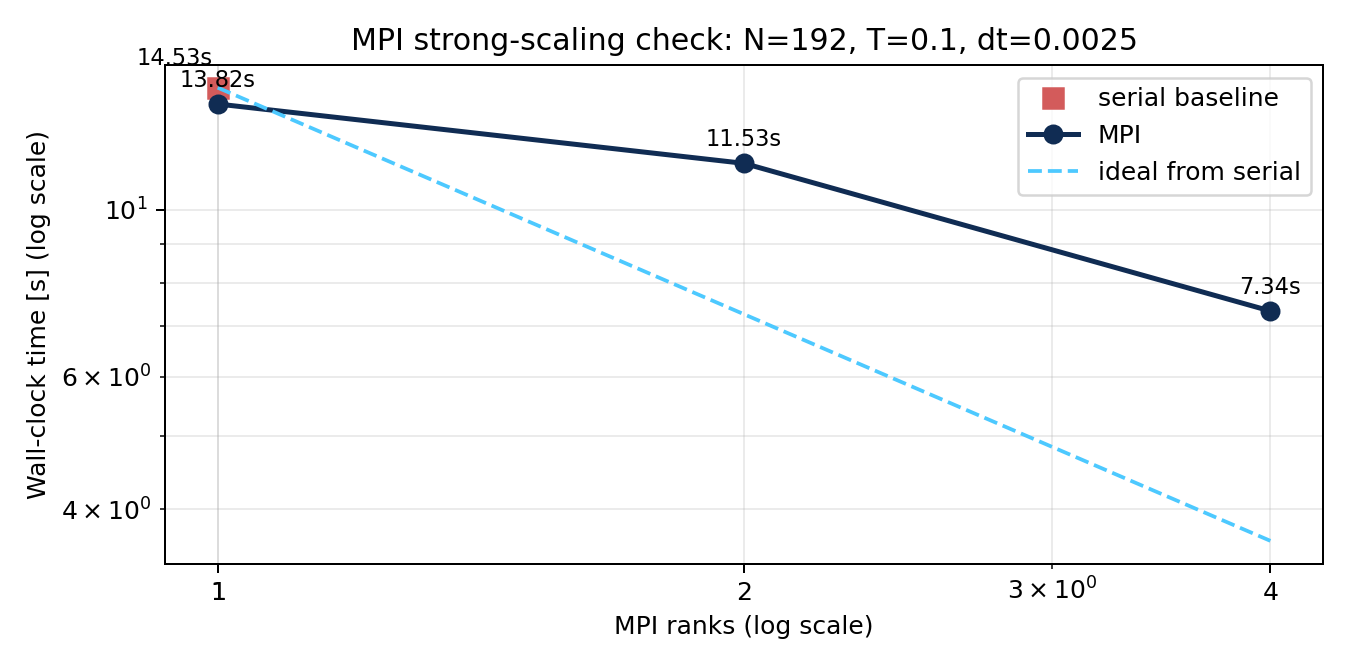
\includegraphics[width=0.78\textwidth]{../../assets/figures/mpi-scaling-loglog.png}
 \caption{End-to-end MPI time versus process count on log--log axes. The
 dashed line is ideal inverse-rank scaling from the one-rank measurement.}
\end{figure}

This is the scalability result obtained in our HPC study, not evidence that the
MPI implementation is missing. It characterises the small-problem regime in
which fixed MPI costs dominate. Increasing the problem size or changing the
machine would let us investigate the complementary strong-scaling regime, but
that is a different experimental regime rather than an unfinished part of the
implementation.

The serial problem-size study in \texttt{run\_scalability\_study.sh} is kept
separate from MPI scaling. Increasing \(N\) there measures the growth of the
serial computational problem; it is not labelled strong or weak scaling.

The validation is intentionally bounded to smooth manufactured standing-wave
data, the unit square and homogeneous Dirichlet conditions. It therefore does
not claim accuracy for nonsmooth data, arbitrary geometries or long-time
propagation.

\small
\begin{thebibliography}{9}
\bibitem{arnold}
D. N. Arnold, D. Boffi, R. S. Falk,
\emph{Approximation by quadrilateral finite elements}.
\url{https://arxiv.org/abs/math/0005036}.
\bibitem{dealii}
deal.II 9.5, \emph{FE\_Q documentation}.
\url{https://dealii.org/9.5.0/doxygen/deal.II/classFE__Q.html}.
Solver and boundary APIs were also checked against the installed 9.5.1 headers.
\bibitem{newmark}
N. M. Newmark, ``A method of computation for structural dynamics,''
\emph{Journal of the Engineering Mechanics Division}, ASCE, 85(EM3),
67--94, 1959.
\bibitem{course}
M. Bucelli, \emph{NMPDE project repository template}.
\url{https://github.com/michelebucelli/nmpde-projects}.
\end{thebibliography}
